
\documentclass{article}
\usepackage[utf8]{inputenc}
\usepackage{graphicx}
\usepackage[T1]{fontenc}
\usepackage{lmodern}
\usepackage{listings}
\usepackage[numbers]{natbib} %IEEE
\usepackage{color}
\usepackage{hyperref}
\usepackage{soul}
\usepackage{float}
\usepackage{pgfplotstable}
\usepackage[font=itshape]{quoting}
\usepackage{booktabs}
\usepackage{amsmath}
\setcounter{MaxMatrixCols}{13}
\usepackage{multicol}
%\usepackage[table,xcdraw]{xcolor}

\usepackage{minted}
\usepackage[a4paper, total={6in, 8in}]{geometry}
\definecolor{dkgreen}{rgb}{0,0.6,0}
\definecolor{gray}{rgb}{0.5,0.5,0.5}
\definecolor{mauve}{rgb}{0.58,0,0.82}
\definecolor{backcolour}{rgb}{0.95,0.95,0.92}
\definecolor{codegreen}{rgb}{0,0.6,0}
% Define a custom style
\lstdefinestyle{myStyle}{
    backgroundcolor=\color{backcolour},   
    commentstyle=\color{codegreen},
    keywordstyle = \bfseries\color{mauve},
    basicstyle=\ttfamily\footnotesize,
    breakatwhitespace=false,         
    breaklines=true,                 
    keepspaces=true,                 
    numbers=left,       
    numbersep=5pt,                  
    showspaces=false,                
    showstringspaces=false,
    showtabs=false,                  
    tabsize=2,
}
\lstset{style=mystyle}

\title{Data Mining \& Machine Learning \\ \large Computer Exercise 8 - Support Vector Machines}
\author{Steinarr Hrafn Höskuldsson}
\date{October 2022}
\newcommand{\mycomment}[1]{}

\begin{document}
\maketitle
\mycomment{
\begin{figure}[h]
    \centering
    \includegraphics[width=0.75\textwidth]{LAB3/Basic1.png}
    \caption{"Switch test" Breadboard set up}
    \label{fig:Switch_test}
\end{figure}

\lstinputlisting[caption=Defining 'ColorMatch' state, label={lst:colormatch}, language=Python, firstline=44, lastline=52]{LAB3/Basic.py}

}
\section*{Section 1.1}
\begin{figure}[H]
    \centering
    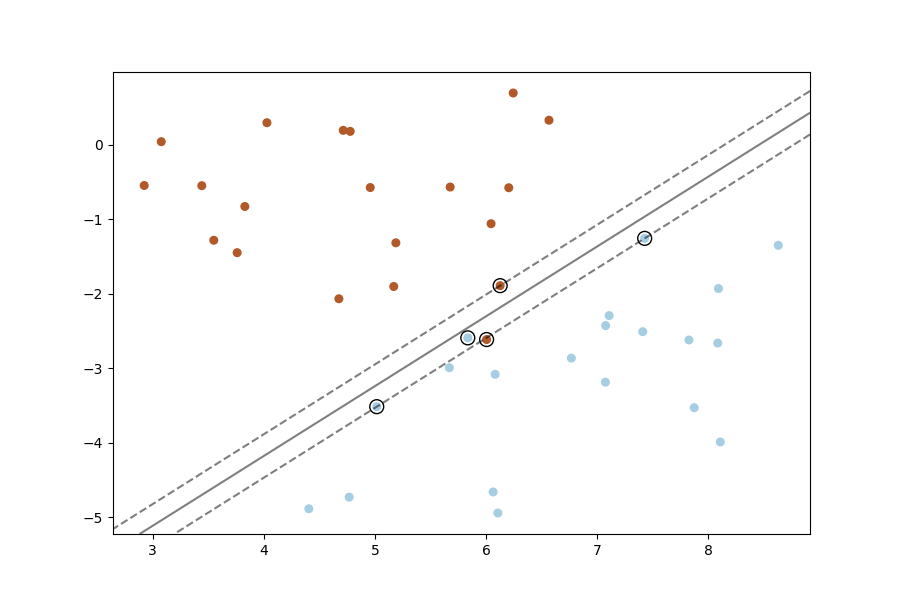
\includegraphics[width=0.75\textwidth]{08_SVM/1_1_1.png}
    \caption{1\_1\_1.png The decision boundary and Support Vector margins for generated data.}
    \label{fig:section11}
\end{figure}

\section*{Section 1.2}
In the support vector machine plotted in Figure \ref{fig:section11} there is one support vector for each of the two classes. Thus the decision boundary is a straight line.

\section*{Section 1.3}
\begin{figure}[H]
    \centering
    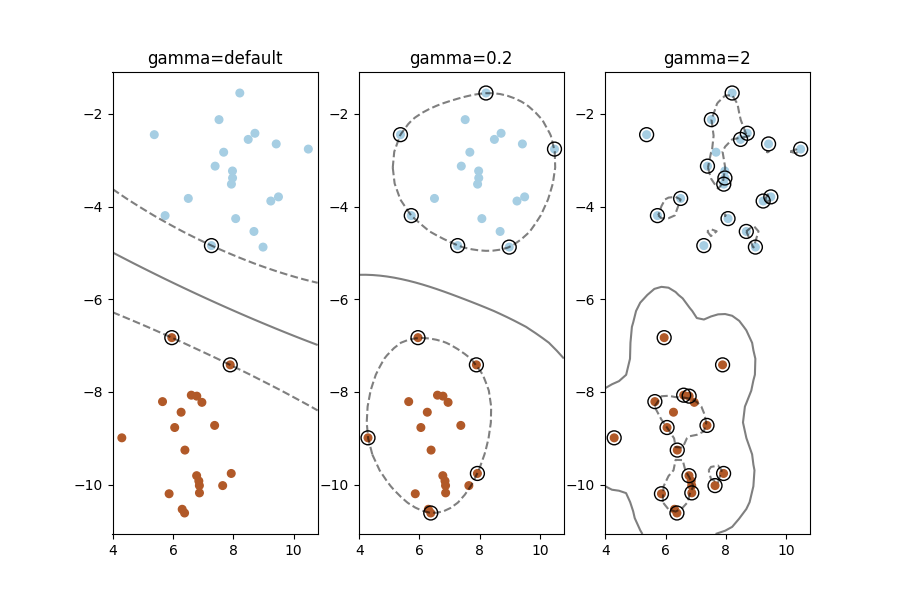
\includegraphics[width=\textwidth]{08_SVM/1_3_1.png}
    \caption{1\_3\_1.png The decision boundary and Support Vector margins for three Support Vector machines that differ only in the value of $gamma$.}
    \label{fig:section13}
\end{figure}

\section*{Section 1.4}
When plotting the decision boundary for different values of gamma as can be seen in Figure \ref{fig:section13} the amount of support vectors were printed:
\begin{verbatim}
For default gamma, number of support vectors is: [1 2]
For gamma=0.2, number of support vectors is: [6 5]
For gamma=2, number of support vectors is: [18 15]
\end{verbatim}

As can be seen on the plots the shape of the decision boundary gets more and more complicated, With default gamma it is a simple curve with a constant curvature, with gamma=0.2 it appears to be a curve with changing curvature and with gamma=2 it is a very complicated shape.

\section*{Section 1.5}
\begin{figure}[H]
    \centering
    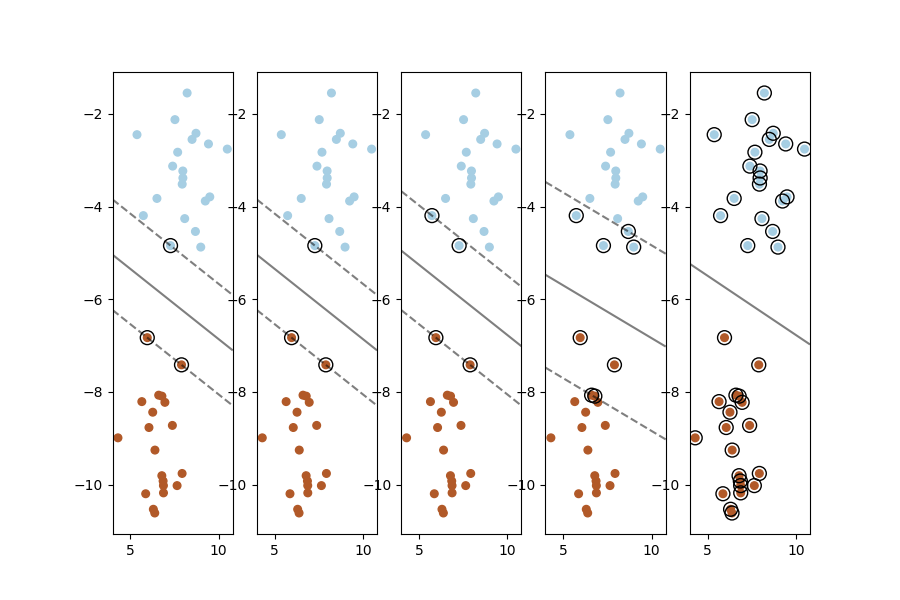
\includegraphics[width=\textwidth]{08_SVM/1_5_1.png}
    \caption{1\_5\_1.png The decision boundary and Support Vector margins for five Support Vector machines that differ only in the value of C}
    \label{fig:section15}
\end{figure}

\section*{Section 1.6}
When plotting the decision boundary for different values of C as can be seen in Figure \ref{fig:section15} the amount of support vectors were printed:
\begin{verbatim}
For C=1000, number of support vectors is: [1 2]
For C=0.5, number of support vectors is: [1 2]
For C=0.3, number of support vectors is: [2 2]
For C=0.05, number of support vectors is: [4 4]
For C=0.0001, number of support vectors is: [20 20]
\end{verbatim}

As C decreases there are more support vectors inside the margins until at $C=0.0001$ all the datapoints are support vectors inside the margins. No support vectors are misclassified although the soft margin classifier being used does allow for that. But since the dataset is linearily seperable it does not occur.

\newpage
\section*{Section 2.2}
The different kernels were tested on the breast cancer dataset. The results can be found in Table \ref{tab:22}
\begin{table}[H]
\centering
\begin{tabular}{llll}
             & Accuracy & Test Score & Recall \\
Linear       & 95.9\%   & 95.4\%     & 97.3\% \\
Radial Basis & 94.7\%   & 94.7\%     & 97.3\% \\
Polynomial   & 93.6\%   & 93.8\%     & 96.4\%
\end{tabular}
\caption{The results of Support Vector machine with different kernels tested on the breast cancer dataset.}
\label{tab:22}
\end{table}
Looking at the results it looks like the linear kernel gave slightly better results.


\section*{Independent}
A collection of monthly average weather observations in Reykjavík from 1949 to 2022 was collected from the Icelandic Meteorological Office's website. The objective being to train a classifier to guess the month based on Average weather observations. A short script was written to parse the values for Average Temperature, Average Pressure, Average Sun hours, Average Wind Speed and The number for the corresponding month. These were then parsed into a train test splitter. 

A Support vector machine was trained on the training data and then made to predict the month from the test data. The Accuracy of the model was around 70\%. Here the confusion matrix can be seen:\\
\\
\begin{bmatrix}
         &Jan. & Feb. & March & April & May & June & July & Aug. & Sept. & Oct. & Nov. & Dec.\\
        January & 6 & 0 & 3 & 3 & 1 & 0 & 0 & 0 & 0 & 0 & 0 & 0\\
February & 0 & 11 & 0 & 0 & 0 & 2 & 0 & 0 & 0 & 0 & 0 & 0\\
March & 0 & 0 & 6 & 0 & 4 & 0 & 0 & 0 & 0 & 0 & 0 & 0\\
April & 1 & 0 & 0 & 15 & 0 & 0 & 0 & 0 & 0 & 0 & 0 & 0\\
May & 0 & 0 & 2 & 0 & 13 & 1 & 0 & 0 & 0 & 0 & 0 & 0\\
June & 0 & 2 & 0 & 0 & 4 & 11 & 0 & 0 & 0 & 0 & 0 & 0\\
July & 0 & 1 & 0 & 0 & 0 & 4 & 10 & 0 & 0 & 0 & 0 & 1\\
August & 0 & 0 & 0 & 0 & 0 & 0 & 2 & 12 & 0 & 0 & 0 & 0\\
September & 0 & 0 & 0 & 0 & 0 & 0 & 0 & 1 & 8 & 0 & 0 & 2\\
October & 0 & 0 & 0 & 0 & 0 & 0 & 0 & 0 & 0 & 13 & 5 & 1\\
November & 0 & 0 & 0 & 0 & 0 & 0 & 0 & 0 & 2 & 10 & 5 & 0\\
December & 0 & 1 & 0 & 0 & 0 & 0 & 0 & 1 & 0 & 0 & 0 & 12
        \end{bmatrix}
\\
\\
\\
More than half inaccuracies are only off by one month and, interestingly, the model seems to have had particular issues with classifying between October and November. 

\newpage
\section*{Appendix}
\appendix
\section{Code}

\lstinputlisting[caption={The code used}, language=Python, ]{08_SVM/Steinarr8.py}



\end{document}

